\documentclass{article}
\usepackage{amsmath,color}
\usepackage{amssymb}
\usepackage{amsfonts}
\usepackage{graphicx}
\usepackage{epsf}
\usepackage{hyperref}
\newtheorem{theorem}{Theorem}
\setlength{\topmargin}{0.1in}
\setlength{\oddsidemargin}{0in}
\setlength{\evensidemargin}{0in}
\setlength{\headheight}{0in}
\setlength{\headsep}{0in}
\setlength{\textheight}{9in}
\setlength{\textwidth}{6.5in}
\renewcommand{\dblfloatpagefraction}{0.9}
\renewcommand{\floatpagefraction}{0.9}
\newenvironment{bibparagraph}{\begin{list}{}{ %
    \setlength{\labelsep}{-\leftmargin} %
    \setlength{\labelwidth}{0pt} %
    \setlength{\itemindent}{-\leftmargin} %
    \setlength{\listparindent}{0pt}}}{\end{list}}
\def\makefigure#1#2{\begin{figure}
\begin{center}
\input{#1}
\end{center}
\caption{#2}
\label{#1}
\end{figure}}

\def\limplies{\; \supset \;}
\def\land{\: \wedge \:}
\def\lor{\: \vee \:}
\def\iff{\; \equiv \;}
\def\lnot{\neg}
\def\lforall#1{\forall \: #1 \;}
\def\lexists#1{\exists \: #1 \;}
\def\glitch#1{{\tt #1}} % glitch on
%\def\glitch#1{} % glitch off
\def\comment#1{}
\def\pnil{[\;]}
\def\pif{\; \mbox{\tt :- } \;}
\def\tuple#1{$\langle #1\rangle$}
\def\mtuple#1{\langle #1\rangle}
\def\ceiling#1{\lceil #1\rceil}
\def\floor#1{\lfloor #1\rfloor}
\def\centerps#1{\begin{center}
\leavevmode
\epsfbox{#1}
\end{center}}
\def\argmax{\mathop{\rm argmax}}
\def\argmin{\mathop{\rm argmin}}
\def\grad{\nabla\!}
\def\celsius{^\circ\mbox{C}}
%\long\def\answer#1{}  % comment out for solutions
%\long\def\question#1{#1} % comment out for solutions
\long\def\answer#1{{\color {blue} { #1}}}  % comment in for solution
\long\def\question#1{} % comment in for solution
%\renewcommand{\labelenumi}{(\alph{enumi})}
%\newcommand{\mbx}{\mathbf{x}}
\newcommand{\mb}[1]{{\mathbf{#1}}}

\def\x{{\bf x}}
\def\w{{\bf w}}

\begin{document}
{
\small
Submitted by: {Oluwasegun Somefun}, somefuno@oregonstate.edu
}
{\Large
\begin{center}
AI534 --- Written Homework Assignment 1 (40 pts) \\ {Due Oct 15th 11:59pm, 2021}
\end{center}
}

%Please submit electronically via TEACH. Your submission should be a single PDF file.

\begin{enumerate}
\item (Weighted linear regression) (15 pts) In class when discussing linear regression, we assume that the Gaussian noise is independently identically distributed. Now we assume the noises $\epsilon_1, \epsilon_2, \cdots \epsilon_n$ are independent but each $\epsilon_i \sim N(0, \sigma_i^2)$, i.e., it has its own distinct variance.

    \begin{enumerate}
    \item (3pts) Write down the log likelihood function of $\mathbf{w}$.\\
    \answer{
    
    Given the likelihood function of $\mathbf{w}$ is $L(\mathbf{w})$:
    
    \[
        L(\mathbf{w}) = \prod_{i=1}^{n} {P\left(y_i\,|\,\mathbf{x}_i, \mathbf{w} \right)}
    \]

    The log-likelihood of $\mathbf{w}$ is therefore
    \[
        l(w) = \log{L(\mathbf{w})} =
    \sum_{i=1}^{n} \log \left[ \frac{1}{\sqrt{2\pi}\,\sigma_i}\, \exp{\left(-\frac{(y_i - \mathbf{w}^T\mathbf{x}_i)^2}{2\,\sigma_i^2}\right)} \right]
    \]

}
    \item (4pts) Show that maximizing the log likelihood is equivalent to minimizing a weighted least square loss function $J(\mathbf{W}) = \frac{1}{2} \sum_{i=1}^na_i(\mathbf{w}^T\mathbf{x}_i-y_i)^2$, and express each $a_i$ in terms of $\sigma_i$.\\
        \answer{

        Maximizing the log-likelihood we have:

    \[ l(w) = \sum_{i=1}^{n} \log \left[ \frac{1}{\sqrt{2\pi}\,\sigma_i} \right]  + \sum_{i=1}^{n} \left[{\left(-\frac{(y_i - \mathbf{w}^T\mathbf{x}_i)^2}{2\,\sigma_i^2}\right)} \right]
    \]

   Therefore,
    \[
    \argmax_{w}{l(w)} =  \argmin_w \frac{1}{2} \sum_{i=1}^{n} { \frac{1}{\sigma_i} \left[ \left(-(y_i - \mathbf{w}^T\mathbf{x}_i)^2 \right) \right] }
    \]

    Setting $a_i = \frac{1}{\sigma_i}$, we have

    \[
      \argmin{J(\mathbf{w})} =  \frac{1}{2} \sum_{i=1}^{n} {a_i}
      {\left( (\mathbf{w}^T\mathbf{x}_i -y_i)^2 \right)}
    \]
    which is equivalent to minimizing a weighted least square loss function, where  $a_i$ is the weights.

}

    \item (4 pts) Derive a batch gradient descent update rule for optimizing this objective.\\
\answer{

        To optimize the objective, the steepest descent gradient rule says to move the weights $\mathbf{w}$ in the direction opposite the gradient of the cost function  $ g = -\nabla_{\mathbf{w}}{J}$, with a suitable step-size $\lambda$

        \[
            \mathbf{w}_{k+1} = \mathbf{w}_k - \Delta \mathbf{w}_k
        \]
        \[
            \Delta \mathbf{w}_k  = -\lambda\,\nabla_{\mathbf{w}}{J\left( \mathbf{w}_k \right)}
        \]
        then repeat for a fixed iteration or till no improvement $|e(\mathbf{w}_k)| \le \epsilon$

        For a vectorized batch gradient descent algorithm, that is, we should sum all the step-directions (gradients) of the $n$ examples before updating the weight is as follows, where $\mathbf{X}$ is a matrix and $e,g,p,w$ are vectors.

        By using the chain rule on the least-square cost-function, the gradient is  $\nabla_{\mathbf{w}}{J\left( \mathbf{w}_k \right)} = \mathbf{g} = \mathbf{X}^T \mathbf{a} \mathbf{e} $, where $ \mathbf{e} = \mathbf{\hat{y} - y} $. The algorithm pseudocode is as follows:

        1. initialize $\mathbf{w} = 0$, $\lambda = \lambda_0$

        2. for each epoch repeat: $k = 1 \hbox{to}\quad k_{\max}$

        3.  $ \mathbf{\hat{y} = \mathbf{X}^{T}\,\mathbf{w}}$

        4.   $ \mathbf{e} = \mathbf{\hat{y} - y} $

        5.   $  \mathbf{g} = \mathbf{X}^T \mathbf{a} \mathbf{e} $

        6.   $ \mathbf{p} = \lambda \mathbf{g}$

        7.   $\mathbf{w} = \mathbf{w} - \mathbf{p} $

        8. end

}
    \item (4 pts) Derive a closed form solution to this optimization problem.\\
    \answer{
    We can also minimize this optimization problem by setting the gradient  to zero. In vectorized form, the gradient is:
    \[
    J\left( \mathbf{w} \right) = \frac{1}{2\,N} \|\mathbf{A\,X\,W} - \mathbf{Y}  \|
    \]
    \[
     \nabla_{\mathbf{w}}{J\left( \mathbf{w} \right)} = 0 =
    {\frac{1}{N},\left( \mathbf{X}^{T}\,\mathbf{A}\,\mathbf{X}\,\mathbf{W} -
     \mathbf{X}\,\mathbf{A}\,\mathbf{Y} \right) }
    \]
    \[
        \mathbf{W} = \left(\mathbf{X}^{T}\,\mathbf{A}\,\mathbf{X} \right)^{-1}\, \mathbf{X}^T\,\mathbf{A}\,\mathbf{Y}
    \]
    which is the normal equation
}
\end{enumerate}
\item (14 pts) Consider the maximum likelihood estimation problem for multi-class logistic regression using the soft-max function defined below:
\[p(y=k|\mathbf{x}) = \frac{\exp(\mathbf{w}_k^T\mathbf{x})}{\sum_{j=1}^K \exp(\mathbf{w}_j^T\mathbf{x})}\]

We can write out the likelihood function as:
\[ L({\mb w})=\prod_{i=1}^N\prod_{k=1}^K p(y=k|{\mb x}_i)^{I(y_i=k)}\] where $I(y_i=k)$ is the indicator function, taking value 1 if $y_i$ is $k$.
\begin{enumerate}
%\item What are $i$ and $k$ in this likelihood function?
%\answer{The first product is over $i = 1$ to $N$ for all instances in the dataset and the second product is for $k = 1$ to $K$ over all classes.}
\item (2 pts) Compute the log-likelihood function.\\
\answer{
 The log-likelihood $l(\mb w)$ is:
\[
l(\mb w) = \log{L({\mb w})} = \sum_{i=1}^N \sum_{k=1}^K {I(y_i=k)}  \log\left( \frac{\exp(\mathbf{w}_k^T\mathbf{x}_i)}{\sum_{j=1}^K \exp(\mathbf{w}_j^T\mathbf{x}_i)} \right)
\]

}
\item  (12 pts) Compute the gradient of the log-likelihood function w.r.t the weight vector ${\mb w}_c$ of class $c$. (Precursor to this question, which terms are relevant for ${\mb w}_c$ in the loglikelihood function? Also hint: Logistic regression slide provides the solution to this problem, just need to fill in what is missing in between.)\\
\answer{

The gradient of $l(\mb w)$ is $\nabla l(\mb w)$. For each $k$, we have:
$\frac{\delta\,l}{\delta\, \mb{w}_k} = \frac{\delta\,l}{\delta\, \hat{y}_{ik}}\,\frac{\delta\,\hat{y}_{ik}}{\delta\, \mb{w}_k}$

 Applying chain rule of calculus, we obtain

\[
    \nabla l(\mb w) = \sum_{i=1}^{N} { \frac{y_{ik}}{\hat{y}_{ik}}\, \frac{\delta\,\hat{y}_{ik}}{\delta\, \mb{w}_k}}
\]
where
\[
    \frac{\delta\,\hat{y}_{ik}}{\delta\, \mb{w}_k} = \left\{
                                                       \begin{array}{ll}
                                                         \mathbf{x}_i\, \hat{y}_{ik} (1 - y_{ij}), & \hbox{if } k = j \hbox{;} \\
                                                         -\mathbf{x}_i\, \hat{y}_{ik}\,y_{ij}, & \hbox{if } k \ne j \hbox{.}
                                                       \end{array}
                                                     \right.
\]
simplifying, we obtain
\[
    \nabla l(\mb w) = \sum_{i=1}^{N} { \left(y_{ik} - \hat{y}_{ik}\right)\,\mathbf{x}_i }
\]

}
\end{enumerate}



\item (11 pts) (Maximum A Posterior Estimation.)
Suppose we observe the values of $n$ IID random variables $X_1, \dots , X_n$ drawn from a single Bernoulli
distribution with parameter $\theta$. In other words, for each $X_i$, we know that $P(X_i = 1) =\theta$ and $P(X_i = 0) = 1- \theta$.
In the Bayesian framework, we treat $\theta$ as a random variable, and use a prior probability distribution over $\theta$ to express our prior knowledge/preference about $\theta$. In this framework,  $X_1, \dots, X_n$ can be viewed as generated by:
\begin{itemize}
\item First, the value of $\theta$ is drawn from a given prior probability distribution
\item Second, $X_1, \dots, X_n$ are drawn independently from a Bernoulli distribution with this $\theta$ value.
\end{itemize}
In this setting, Maximum A Posterior (MAP) estimation is a natural way to estimate the value of $\theta$ by choosing the most probable value given both its prior distribution and the observed data $X_1, \dots , X_n$. Specifically, the MAP estimation of $\theta$ is given by
%\begin{equation}
\begin{align*}
\hat{\theta}_{MAP} & = \argmax_{\hat{\theta}}P(\theta=\hat{\theta}|X_1,\dots, X_n)\\
&=\argmax_{\hat{\theta}}P(X_1,\dots,X_n|\theta = \hat{\theta} )P(\theta=\hat{\theta})\\
& = \argmax_{\hat{\theta}}L(\hat{\theta})p(\hat{\theta})
\end{align*}
%\end{equation}
where $L(\hat{\theta})$ is the data likelihood function and $p(\hat{\theta})$ is the density function of the prior.  Now consider using a beta distribution for prior: $\theta ~ Beta(\alpha, \beta)$, whose PDF function is
\[p(\hat{\theta}) = \frac{\hat{\theta}^{(\alpha-1)}(1-\hat{\theta})^{(\beta-1)}}{B(\alpha, \beta)}\]
where $B(\alpha, \beta)$ is a normalizing constant to make it a proper probability density function.

\begin{enumerate}
\item (5 pts) Derive the posterior distribution $p(\hat{\theta}|X_1, \dots, X_n, \alpha, \beta)$ and show that it is also a Beta distribution.\\
\answer{

Let $p(\hat{\theta}|X_1, \dots, X_n, \alpha, \beta) = P(\hat{\theta}|D)$, where $D$ represent the data drawn from a single bernoulli distribution.

The posterior distribution can be written as:
\[
P(\hat{\theta}|D) = P(D|\hat{\theta})\,P(\hat{\theta})
\]
where
\[
P(D|\hat{\theta}) = \left(
                      \begin{array}{c}
                        n \\
                        k \\
                      \end{array}
                    \right)
 \hat{\theta}^{(k)}(1-\hat{\theta})^{(1-k)}
\]
 and
\[
P(\hat{\theta}) = \frac{\hat{\theta}^{(\alpha-1)}(1-\hat{\theta})^{(\beta-1)}}{B(\alpha, \beta)}
\]
which leads to
\[
P(\hat{\theta}|D) = \left(
                      \begin{array}{c}
                        n \\
                        k \\
                      \end{array}
                    \right) \frac{\hat{\theta}^{((k+\alpha)-1)}(1-\hat{\theta})^{((n-k+\beta)-1)}}{B(\alpha, \beta)}
\]

Since both $\left(
                      \begin{array}{c}
                        n \\
                        k \\
                      \end{array}
                    \right)$ and  $ B(\alpha, \beta) = \frac{\Gamma(\alpha+\beta)}{\Gamma(\alpha)\,\Gamma(\beta)} $ are factorial functions  leading to a constant, we have

\[P(\hat{\theta}|D) \propto Beta({(k+\alpha)}, {(n-k+\beta)})\]

which proves that the posterior distribution is also a beta distribution.
}

\item (6 pts) Suppose we use $Beta(2,2)$ as the prior, What is the posterior distribution of $\theta$ after we observe $5$ coin tosses and $2$ of them are head? What is the posterior distribution of $\theta$ after we observe $50$ coin tosses and $20$ of them are head? Plot the pdf function of these two posterior distributions. Assume that $\theta=0.4$ is the true probability, as we observe more and more coin tosses from this coin, what do you expect to happen to the posterior?\\
\answer{
Using, the posterior distribution definition above, let the number of iid samples with a bernoulli distribution, in form of coin tosses be $n$, let the number of observations be $k$ heads and $n-k$ tails.

Starting with the assumption of a fair coin as a prior $Beta(\alpha, \beta) = Beta(2,2)$, and $\theta=0.4$

 For $n=5, k=2$ we have
\[
P(\hat{\theta}|D) =  \left(
                      \begin{array}{c}
                        5 \\
                        2 \\
                      \end{array}
                    \right)\frac{\hat{\theta}^{(3)}(1-\hat{\theta})^{(4)}}{B(2,2)} %= 0.4977
\propto Beta(4,5)
\]

 For $n=50, k=20$ we have
\[
P(\hat{\theta}|D) =   \left(
                      \begin{array}{c}
                        50 \\
                        20 \\
                      \end{array}
                    \right)\frac{\hat{\theta}^{(21)}(1-\hat{\theta})^{(31)}}{B(2,2)}  %= 0.1650
\propto Beta(22,32)
\]

The Probability Distribution Function (PDF) plot of the two posteriors is shown in Fig.\ref{betapdf_fig}.

\begin{figure}[!h]
  \centering
  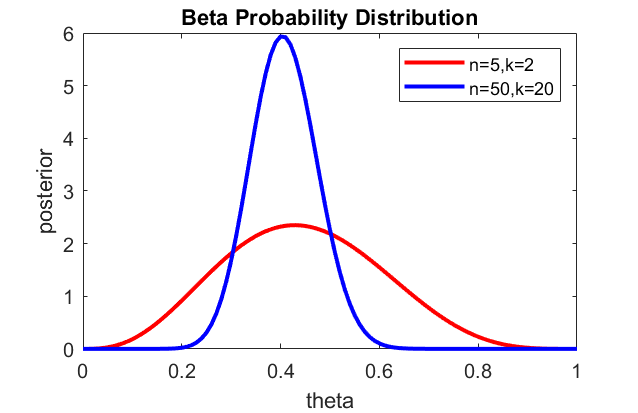
\includegraphics[width=0.5\linewidth]{betapdfs.png}
  \caption{PDF plot of the two Posterior distributions}\label{betapdf_fig}
\end{figure}

As we observe more and more coin tosses, from Fig~\ref{betapdf_fig}, we expect the posterior to converges to the true value which is the mode of the posterior distribution, that is  $\hat{\theta}_{MAP} \approx 0.4$. This can be proved using the following formula, and substituting for $n,k, \alpha,\beta$
\[
\hat{\theta}_{MAP}= \frac{k +(\alpha-1)}{ n + (\alpha + \beta)-2}
\]

}
\end{enumerate}
\end{enumerate}
\end{document}
